\section{Urnenmodelle}

Ein ``Urnenmodell'' ist eine abstrakte Darstellung von Zufallsexperimenten, bei denen zufällig Stichproben aus einer gegebenen Menge ``gezogen'' werden.
Eine Urne ist ein Behältnis in welchem sich farbige/nummerierte Kugeln befinden, die ansonsten ununterscheidbar sind.
Aus der Urne ziehe man blind/zufällig eine oder mehrere Kugeln und notiere ihre Farbe/Zahl.

\begin{center}
    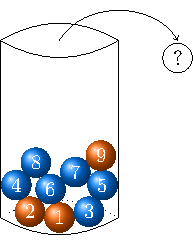
\includegraphics{./stoch_abbildungen/urne_mit_kugeln.pdf}
    \captionof{figure}{Urnenmodell mit nummerierten, farbigen Kugeln}
\end{center}

\subsection{Urnenmodell mit Zurücklegen: Multinomial-Verteilung}

Gegeben sei eine Urne mit $N$ Kugeln, verschiedenfarbig mit Farben aus $E$, wobei $\abs{E} \ge 2$ 

Man ziehe $n$ Stichproben/Kugeln, wobei nach jedem Zug die Kugel wieder zurückgelegt wird. Uns interessiert die Farbe in jedem Zug, setze also
\begin{equation*}
	\Omega = E^n \und \ereignisF = \pows(\Omega) 
\end{equation*}
Zur Bestimmung eines geeigneten Wahrscheinlichkeitsmaßes nummerieren wir die Kugeln mit $1,\dots, N$, so dass alle Kugeln der Farbe $a \in E$ eine Nummer aus $F_{a} \subset \menge{1,\dots, N}$ tragen. Würden wir die Nummern notieren, so wäre
\begin{equation*}
	\quer{\Omega} = \menge{1,\dots, N}^n \und \quer{\ereignisF} = \pows(\quer{\Omega})
\end{equation*}
und wir könnten die Gleichverteilung $\quer{\P} = U(\quer{\Omega})$ als WMaß für einem einzelnen Zug verwenden. Für den Übergang zu $\Omega$ konstruieren wir  Zufallsvariablen. Die Farbe im $i$-ten Zug wird beschrieben durch
\begin{equation*}
	\bigabb{X_i}{\quer{\Omega}}{E}{\quer{\omega} = \left( \quer{\omega}_1, \dots, \quer{\omega}_n \right)}{a \enskip \text{ falls } \quer{\omega}_i \in F_a}
\end{equation*}
Der Zufallsvektor
\begin{equation*}
	\abb{X = (X_1, \dots, X_n)}{\quer{\Omega}}{\Omega}
\end{equation*}
beschreibt dann die Abfolge der Farben. Für jedes $\omega \in \Omega$ gilt dann
\begin{equation*}
	\menge{X = \omega} = F_{\omega_1} \times \cdots \times F_{\omega_n} = \bigtimes_{i=1}^{n} F_{\omega_i}
\end{equation*}
und damit
\begin{equation*}
	\begin{aligned}
    \P(\menge{\omega}) 
    &= \quer{\P}(X^{-1}(\menge{\omega})) = \P(X=\omega)\\
    &= \frac{\abs{F_{\omega_1}} \cdots \abs{F_{\omega_n}}}{\abs{\quer{\Omega}}}\\
    &= \prod_{i=1}^{n} \frac{\abs{F_{\omega_i}}}{N} \\
    &\defqe \prod_{i=1}^{n} \rho(\omega_i)
    \end{aligned}
\end{equation*}
Zähldichten, die sich als Produkt von Zähldichten schreiben lassen, werden auch als \begriff{Produktdichten} bezeichnet ($\nearrow$  \S 3 Unabhängigkeit).

Sehr oft interessiert uns bei einem Urnenexperiment nicht die Reihenfolge der gezogenen Farben, sondern nur die Anzahl der Kugeln in Farbe $a \in E$ nach $n$ Zügen. Dies enspricht
\begin{equation*}
	 \dach{\Omega} 
	 = \menge{k = (k_a)_{a \in E} \in \N_{0}^{\abs{E}} \colon \sum_{a \in E} k_a = n}
	 \und \dach{\ereignisF} = \pows{\dach{\Omega}}
\end{equation*}
Den Übergang $\Omega \to \dach{\Omega}$ beschreiben wir durch die Zufallsvariablen
\begin{equation*}
	\bigabb{Y_a(\omega)}{\Omega}{\N_{0}}%
    {\omega = (\omega_1,\dots, \omega_n)}%
    {\sum_{a \in E} \one_{\menge{a}}(\omega_i)}
\end{equation*}
und
\begin{equation*}
	\abb{Y = (Y_a)_{a \in E}}{\Omega}{\dach{\Omega}}
\end{equation*}